% Meeting brief, 4 November 2026 -- two pages, for the discussion with the professor
\documentclass[10pt,a4paper]{article}
\usepackage[utf8]{inputenc}
\usepackage[T1]{fontenc}
\usepackage{lmodern}
\usepackage[margin=1.6cm,top=1.4cm,bottom=1.5cm]{geometry}
\usepackage{amsmath,booktabs,graphicx,xcolor,tabularx,enumitem}
\usepackage[hidelinks]{hyperref}
\graphicspath{{../figures/}{figures/}}
\pagestyle{empty}
\setlength{\parindent}{0pt}
\definecolor{accent}{HTML}{2B6CB0}
\definecolor{ok}{HTML}{2F855A}
\definecolor{warn}{HTML}{C05621}
\newcommand{\ok}{\textcolor{ok}{\textbf{OK}}}
\newcommand{\warn}{\textcolor{warn}{\textbf{Issue}}}
\newcommand{\head}[1]{\vspace{0.5em}{\large\bfseries\color{accent}#1}\par\vspace{0.25em}}
\newcommand{\answer}{\par\vspace{0.1em}{\small\color{gray}Your answer: \hrulefill}\par\vspace{0.35em}}

\begin{document}

{\LARGE\bfseries Swiss CPI inflation forecast, 2026Q4--2029Q3}\\[0.2em]
{\small Martin Sinishta, Yanik Bittel, Evan Weihs \quad$\cdot$\quad Meeting of 4 November 2026 \quad$\cdot$\quad Details in the technical report}

\vspace{0.6em}
\fcolorbox{accent}{accent!6}{\parbox{\dimexpr\textwidth-2\fboxsep-2\fboxrule}{\small
\textbf{Where we are.} Headline inflation is forecast at \textbf{0.9\% in 2026Q4}, settling at \textbf{about 0.45\%} from mid-2027.
A permanent Brent +50\% shock adds \textbf{+0.4 pp for one year}. Out of sample (55 origins since 2012) the forecasts are
\textbf{unbiased} and \textbf{beat a headline ARIMA and a random walk at 2--3 years}, but are \textbf{not efficient beyond one year}.}}

\head{1. Models: estimated on 2000Q1--2026Q3, $y = 100\ln(\text{index})$}
{\small
\begin{tabularx}{\textwidth}{@{}l r l X l@{}}
  \toprule
  Block & Weight & Model & Key estimates & \\
  \midrule
  Domestic excl.\ rents & 59\% & ARIMA(0,1,0)(1,0,0)$_4$ & drift 0.6\%/yr; seasonal AR 0.73; Ljung--Box $p=0.11$ & \ok \\
  Imported excl.\ oil & 20\% & ARIMA(2,1,1)(1,0,0)$_4$ & drift $-0.6$\%/yr (n.s.); AR root $-0.98$ cancels MA root $-0.74$ & \warn \\
  Rents & 19\% & ARIMA(1,1,1)(1,0,0)$_4$ & drift 1.4\%/yr; all coefficients significant; LB $p=0.74$ & \ok \\
  Oil products & 2\% & ECM & long run: Brent 0.43, CHF/USD 0.61, trend 1.7\%/yr; 39\% of gap closed per quarter & \ok \\
  \bottomrule
\end{tabularx}}

\vspace{0.3em}
{\small Checks: optimal-forecast recursions coded from our derivations = R's \texttt{predict()} (to $10^{-13}$); blocks re-aggregate to headline within 0.14 pp; Engle--Granger cointegration yes, Johansen no (same long-run vector).}

\head{2. Forecast and out-of-sample record}
\begin{minipage}[t]{0.49\textwidth}
  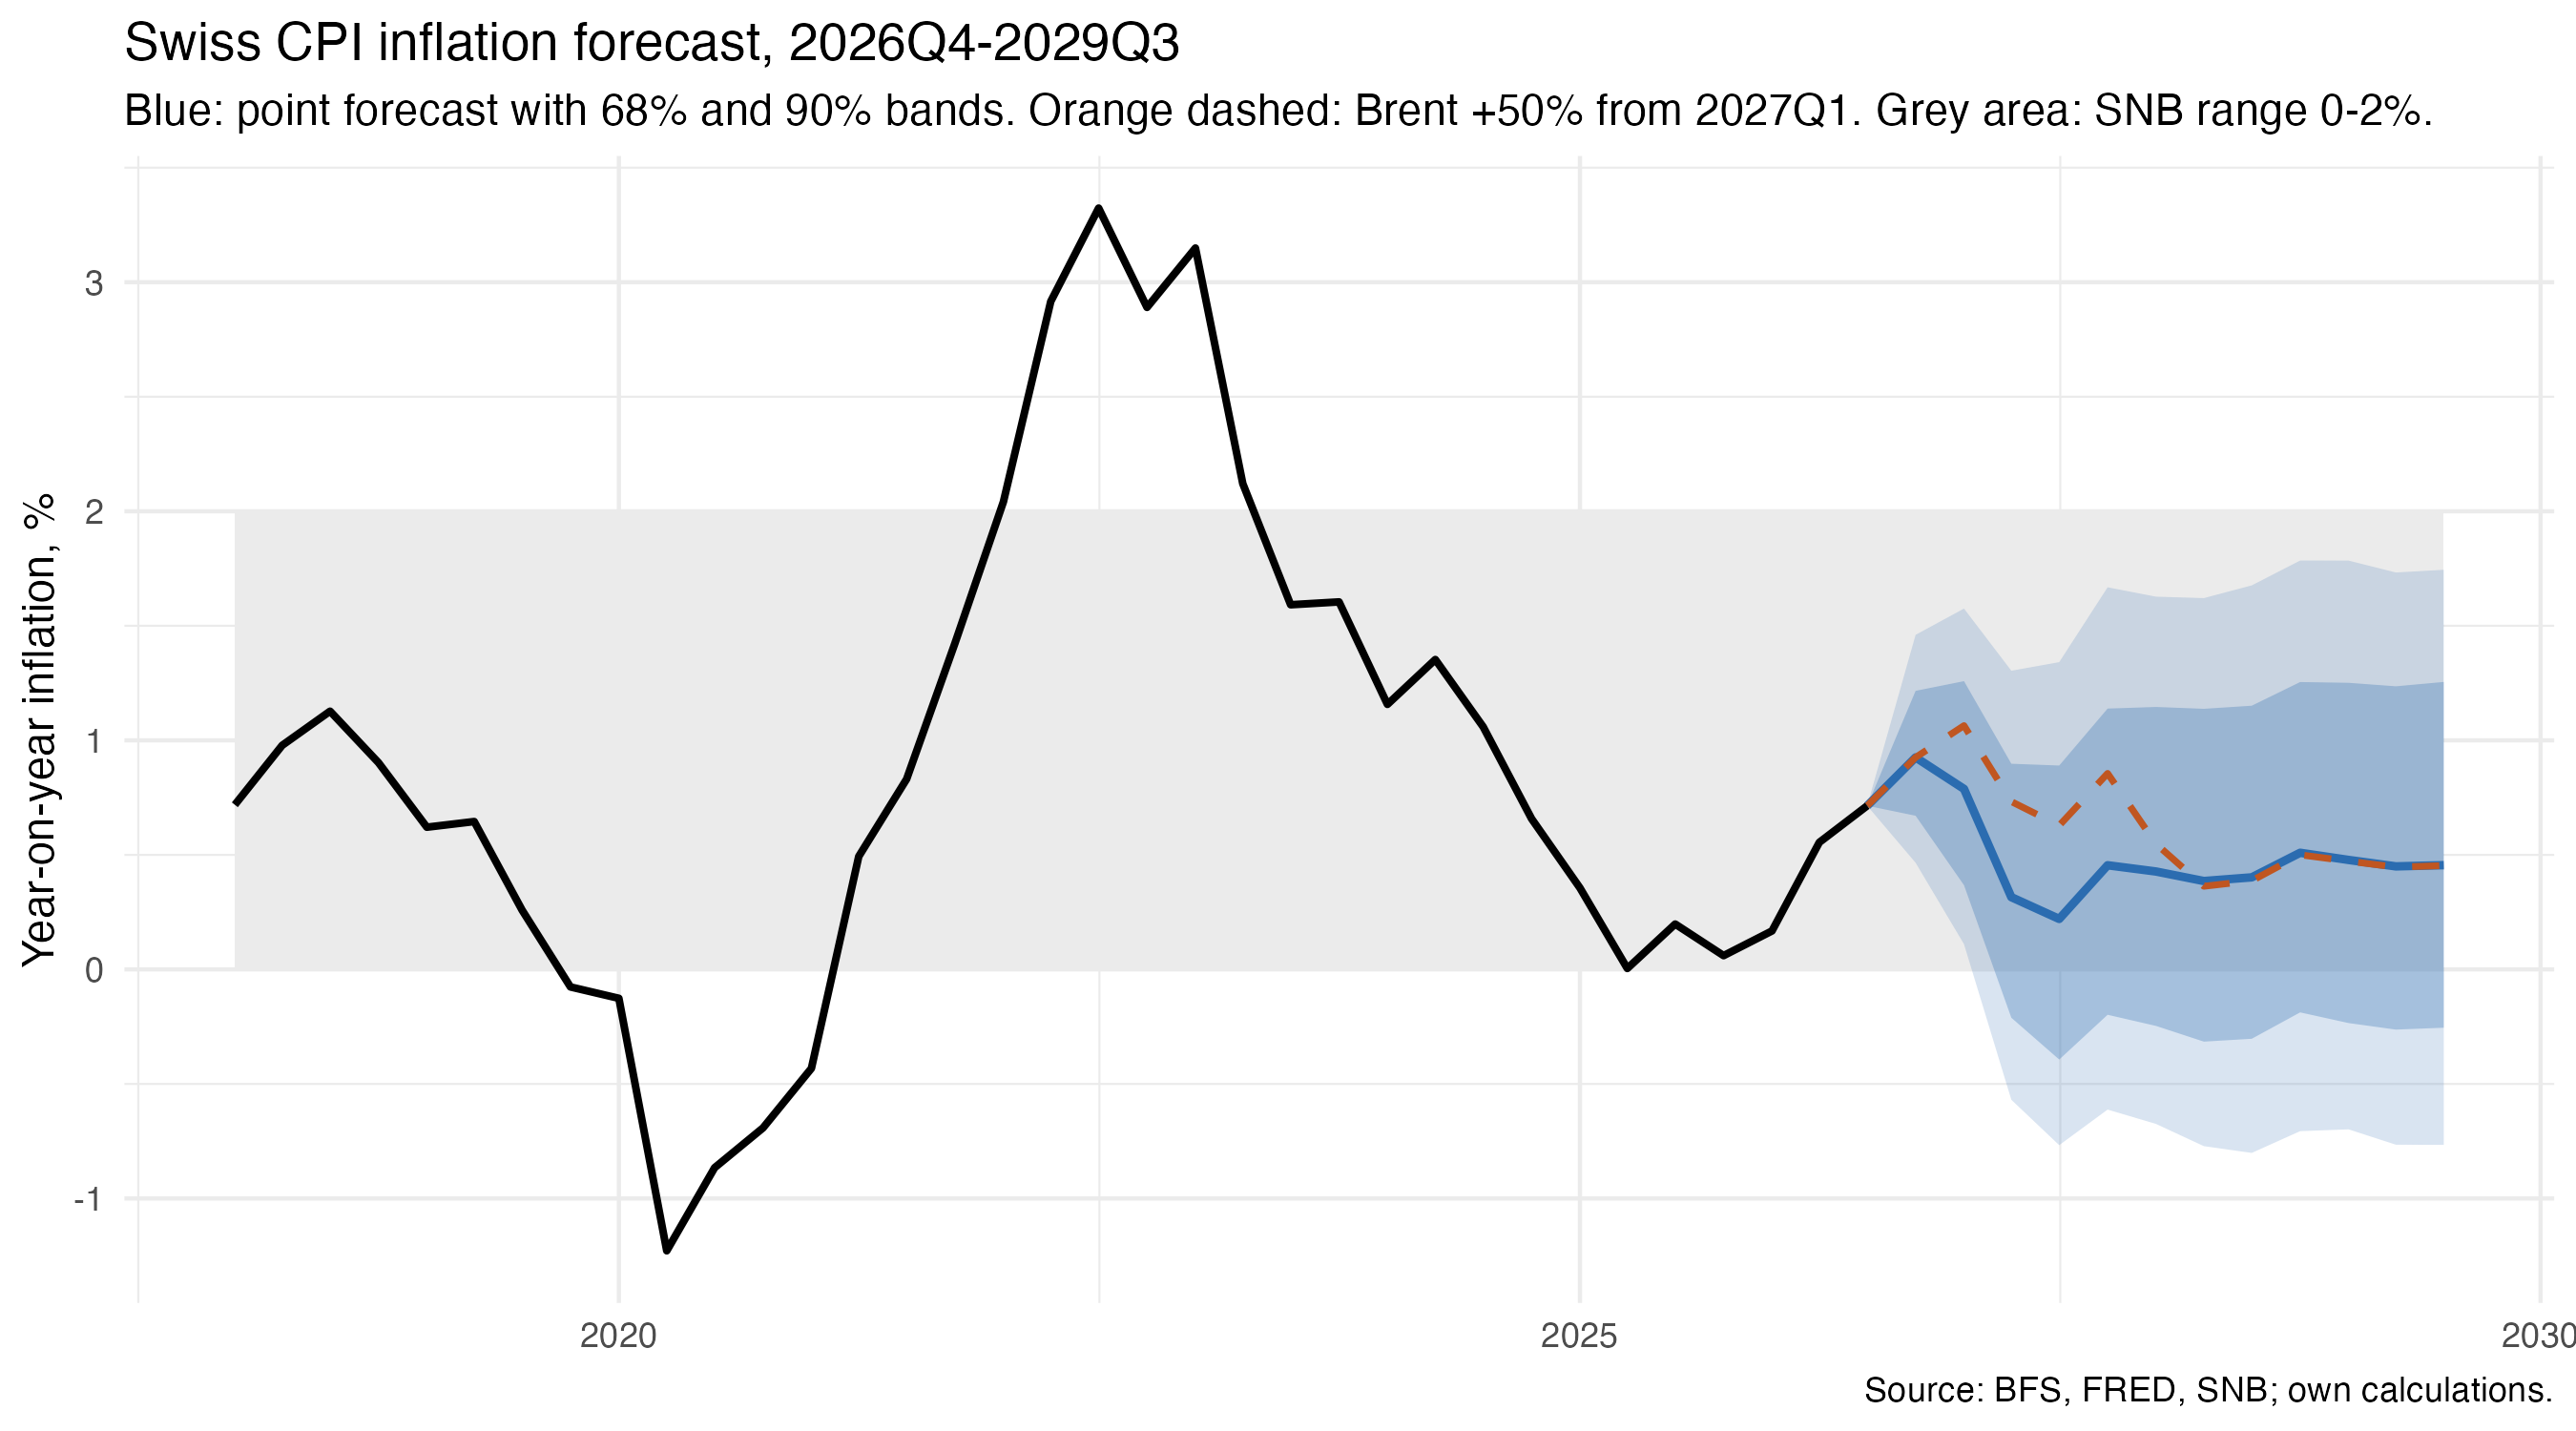
\includegraphics[width=\linewidth]{fan_chart_headline}
\end{minipage}\hfill
\begin{minipage}[t]{0.49\textwidth}
  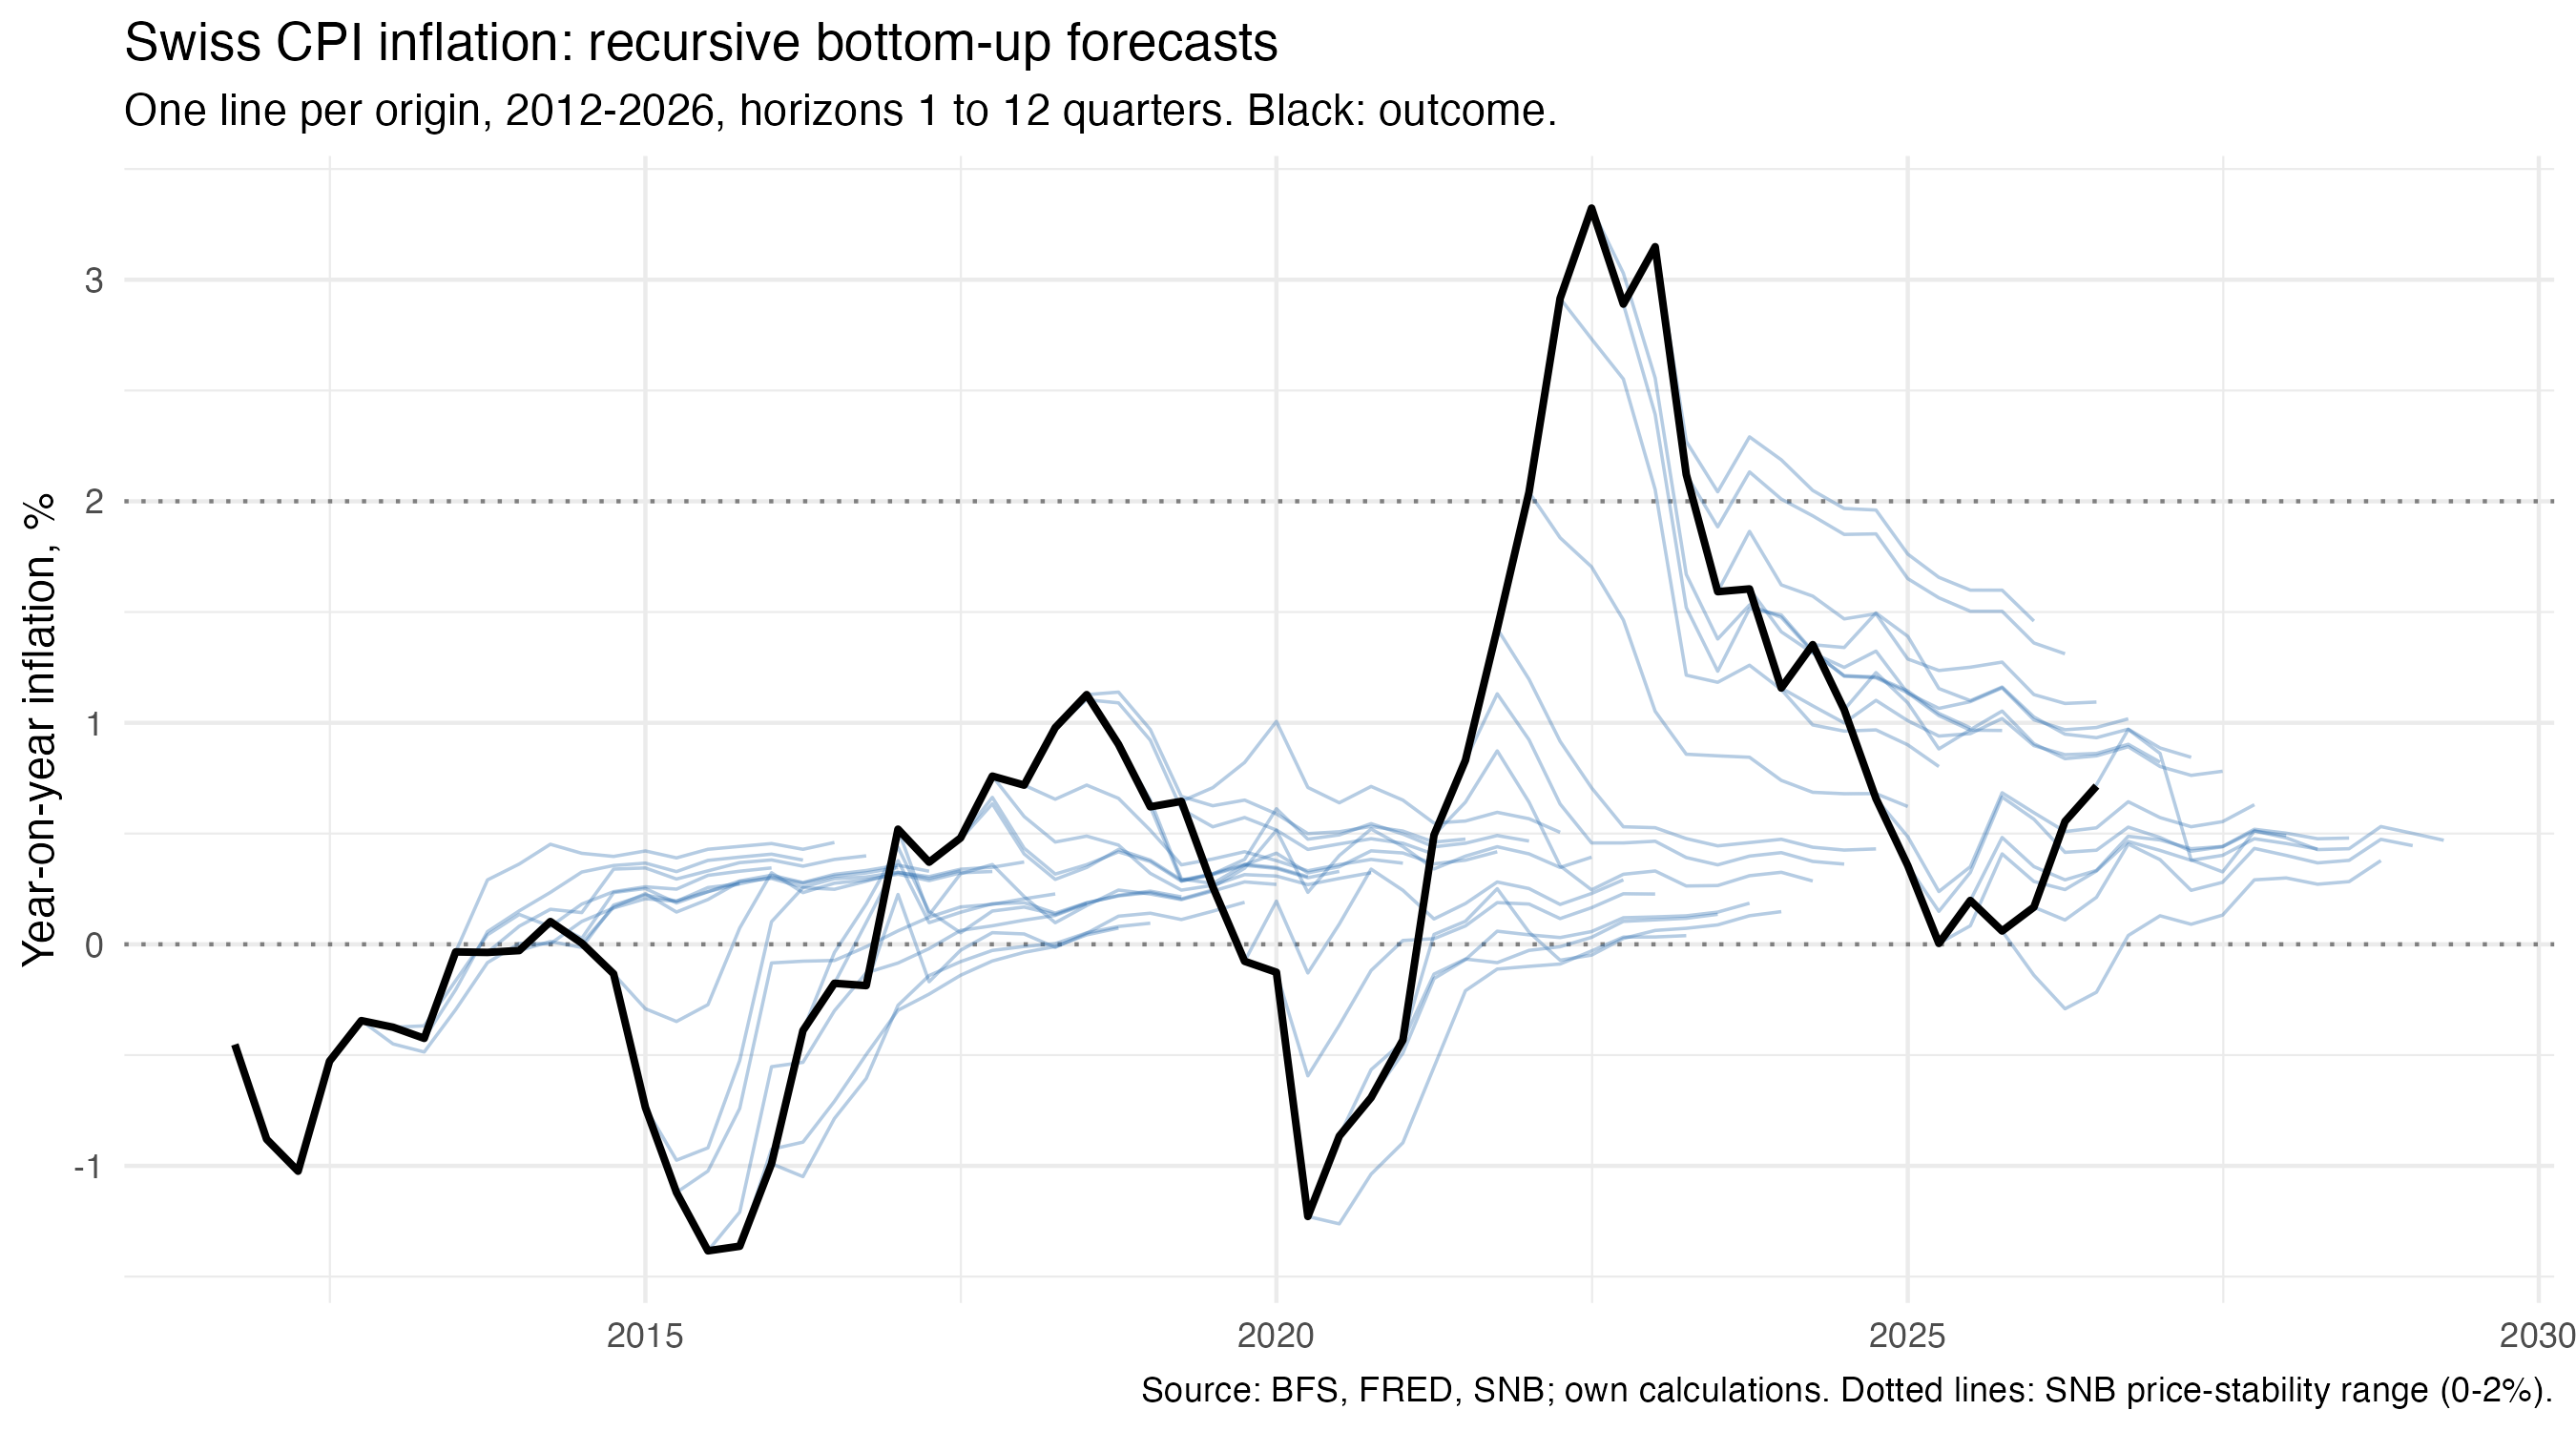
\includegraphics[width=\linewidth]{spaghetti_headline}
\end{minipage}

\vspace{0.3em}
{\small
\begin{tabularx}{\textwidth}{@{}X cccc@{}}
  \toprule
  Horizon $h$ (quarters) & 1 & 4 & 8 & 12 \\
  \midrule
  RMSE, pp & 0.36 & 1.06 & 1.29 & 1.20 \\
  Unbiased ($p$) & 0.71 & 0.90 & 0.84 & 0.50 \\
  Mincer--Zarnowitz ($p$) / strong efficiency ($p$) & 0.65 / 0.01 & 0.36 / 0.04 & 0.01 / 0.01 & 0.00 / 0.00 \\
  MSFE ratio vs headline ARIMA (DM $p$) & 0.99 (0.97) & 1.04 (0.80) & \textbf{0.80} (0.04) & \textbf{0.75} (0.04) \\
  MSFE ratio vs random walk (DM $p$) & 0.78 (0.29) & 0.84 (0.39) & \textbf{0.56} (0.02) & 0.46 (0.07) \\
  \bottomrule
\end{tabularx}}

\vspace{0.2em}
{\small \textbf{Reading:} no bias; disaggregation pays off at 2--3 years; beyond one year the model extrapolates
the current situation and misses turning points (2022 surge, 2024--25 fall), so efficiency is rejected.}

\head{3. Code}
{\small
\begin{tabularx}{\textwidth}{@{}l X@{}}
  \texttt{main.R} & All parameters in one place; runs the pipeline; one run (30 s) reproduces every table and figure \\
  \texttt{01}--\texttt{02} & Data from APIs (BFS, FRED, SNB), never edited by hand; block indices built per annual chain link; quarterly averages \\
  \texttt{04\_model\_estimation} & \texttt{stats::arima} (ML), \texttt{lm}, \texttt{urca}; no auto-selection; diagnostics, cointegration, checks \\
  \texttt{05\_forecasting} & Hand-coded recursions \texttt{arima\_paths()}, \texttt{ecm\_paths()}; 5,000 joint simulated paths; scenario \\
  \texttt{06\_evaluation} & Recursive loop re-estimating at 55 origins; own MZ, efficiency and DM tests with Newey--West errors \\
\end{tabularx}}

\newpage
% ==========================================================================
\head{4. Decisions we need from you}
{\small Each point: what we propose, why, and the alternative.}

\begin{enumerate}[leftmargin=1.4em, itemsep=0.1em]
  \item \textbf{Seasonality.} The non-oil models have a seasonal AR term (so SARIMA).
        \emph{We propose:} test for seasonality, adjust with X-13 where present, then plain ARIMA (TA's advice);
        the y-y target is unaffected. \emph{Alternative:} keep the seasonal AR term and justify it.
        \answer
  \item \textbf{Cointegration.} Engle--Granger: $-5.30 < -4.10$ (cointegrated). Johansen trace: $37.98 < 42.44$ (not).
        \emph{We propose:} keep the ECM, report both; the two give the same long-run vector.
        \emph{Alternative:} ARDL bounds test.
        \answer
  \item \textbf{ECM trend.} Oil products drift up 1.7\%/yr for given Brent and CHF/USD; with random-walk drivers
        the oil forecast is the trend alone after a year. \emph{We propose:} keep it (taxes, CO$_2$ levy).
        \emph{Alternative:} CO$_2$-levy step dummies instead of a trend.
        \answer
  \item \textbf{Brent and CHF/USD.} \emph{We propose:} random walk, plus a Brent shock scenario for the SNB.
        \emph{Alternative:} the futures curve (market-based, but no free API).
        \answer
  \item \textbf{Imported block.} The negative drift ($-0.14$/quarter, n.s., from the 2009--16 strong franc) lowers
        headline by 0.13 pp over the whole horizon; AR and MA roots nearly cancel.
        \emph{We propose:} drop the drift and estimate ARIMA(1,1,0) or (0,1,1).
        \emph{Alternative:} 2009--2016 dummy, or a later sample start.
        \answer
  \item \textbf{Density bands.} The 90\% half-width at $h=8$ is 1.24 pp, while the out-of-sample RMSE implies about 2.1 pp.
        \emph{We propose:} evaluate coverage, then calibrate the bands on out-of-sample errors.
        \emph{Alternative:} add parameter uncertainty by bootstrap.
        \answer
  \item \textbf{Weights before 2016.} Recovered from the CPI identity by least squares (error $\le$ 0.04 pp against
        published 2016--26 weights). \emph{We propose:} use them. \emph{Alternative:} published series only, from 2016.
        \answer
\end{enumerate}

\head{5. Next steps}
{\small
\begin{itemize}[leftmargin=1.4em, itemsep=0.05em]
  \item Script 03: unit-root tests (deterministic vs stochastic trend for domestic), seasonality plots, X-13.
  \item Re-estimate the non-oil blocks as plain ARIMA; simplify the imported model; additive outliers for COVID and 2022.
  \item Density forecast evaluation (coverage, PIT); rerun the evaluation with the revised models.
  \item Minto pyramid of the statement; technical and non-technical reports.
\end{itemize}}

\vspace{0.4em}
{\small\color{gray}Notes:}\par
\newcommand{\noteline}{\par\vspace{1.3em}{\color{gray!60}\rule{\textwidth}{0.3pt}}}
\noteline\noteline\noteline\noteline\noteline\noteline\noteline

\end{document}
